\section{Description and Methodology}

\subsection{Compiling the Linux kernel}
We were supplied with a variant of Linux called \emph{uClinux}, and it's supplied toolchain. We built the distribution by using a build system named \emph{ptxdist}. We followed \cite[section 5.3]{compendium} step by step, and when done we ended up with a working linux distribuion on the chip, with Tux drawn on the screen. Initially we did not change the kernel config\footnote{We ended up doing so, please see section \ref{subsection:energy-efficiency}.}, nor add any more packages than already configured.

\subsection{Device driver for the gamepad}

\subsection{Signals and interrupts}
\label{subsection:signals-and-interrupts}

\subsection{Controlling the screen}

\subsection{Pong}

\subsection{Energy efficiency}
\label{subsection:energy-efficiency}
As we are no longer programming on the "bare metal", we have less control over the software running on the chip. \emph{uClinux} have certain requirements regarding timers and other peripherals, and \cite{compendium} states that "all relevant clocks are already turned on", which we consider as a statement that says the oscilator setup is fixed, and should not be altered for this exercise.

\subsubsection{Interrupts and signals}
We implemented our driver so no polling mechanisms were needed (as described in section \ref{subsection:signals-and-interrupts}). As a consequence, the program will stay most of its time in a \emph{pause()} loop, leaving the CPU and IO buses free to do other stuff, or in this case, sleep. This behaviour decreases power consumption.

\subsubsection{Optimizing screen update}


\subsubsection{Tickless idle}
\begin{figure}[h]
	\centering
	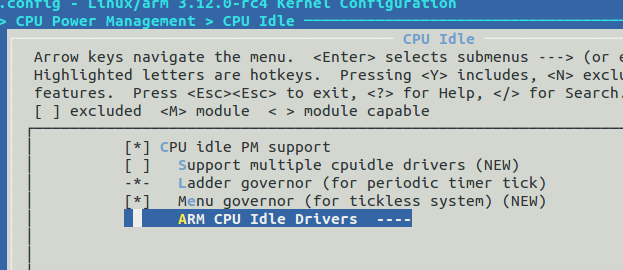
\includegraphics[width=12cm]{img/tickless.png}
	\caption{Configuring the kernel to tickless idle}
	\label{fig:tickless}
\end{figure}
Because our game is handeled entirely by signal handlers, leaving the main program in a pause loop, we wanted to reduce the power consumption while waiting for an interrupt/signal. In order to do that, we were adviced to put the kernel in a mode known as tickless idle. We did this by setting
